\documentclass[border=4pt]{standalone}
\usepackage{tikz}
\usepackage{pgfplots}
\pgfplotsset{compat=1.18}
\usetikzlibrary{shapes.geometric,arrows.meta,positioning,calc,fit,decorations.pathreplacing,backgrounds}
\definecolor{boxblue}{RGB}{225,238,252}
\definecolor{boxgreen}{RGB}{225,247,231}
\definecolor{boxorange}{RGB}{253,236,216}
\definecolor{boxgray}{RGB}{237,237,237}
\definecolor{boxred}{RGB}{253,226,226}
\begin{document}
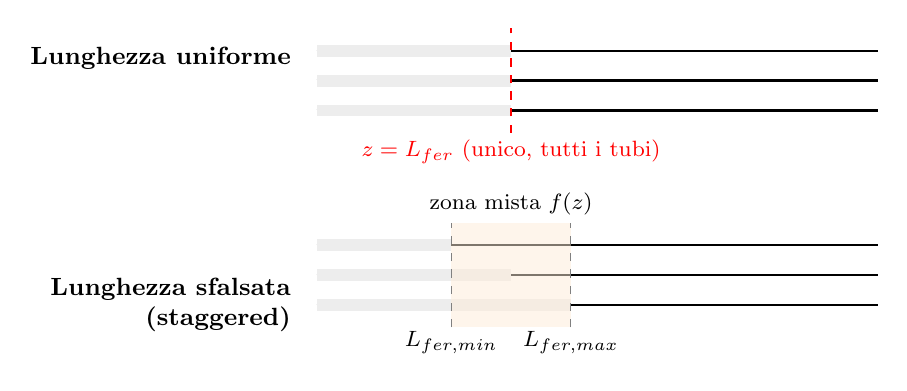
\begin{tikzpicture}[scale=0.95]
% --- Uniform case (top) ---
\node[font=\small,align=right,anchor=east,fill=white,inner sep=1pt] at (-0.3,2.3) {\textbf{Lunghezza uniforme}};
\foreach \y in {1.6,2.0,2.4}{
  \draw[thick] (0,\y) -- (7.5,\y);
}
\foreach \y in {1.6,2.0,2.4}{
  \fill[boxgray] (0,\y-0.08) rectangle (2.6,\y+0.08);
}
\draw[dashed,red] (2.6,1.3) -- (2.6,2.7);
\node[font=\footnotesize,red] at (2.6,1.05) {$z=L_{fer}$ (unico, tutti i tubi)};

% --- Staggered case (bottom) ---
\node[font=\small,align=right,anchor=east,fill=white,inner sep=1pt] at (-0.3,-1.0) {\textbf{Lunghezza sfalsata}\\ \textbf{(staggered)}};
\draw[thick] (0,-0.2) -- (7.5,-0.2);
\fill[boxgray] (0,-0.28) rectangle (1.8,-0.12);
\draw[thick] (0,-0.6) -- (7.5,-0.6);
\fill[boxgray] (0,-0.68) rectangle (2.6,-0.52);
\draw[thick] (0,-1.0) -- (7.5,-1.0);
\fill[boxgray] (0,-1.08) rectangle (3.4,-0.92);
\fill[boxorange,opacity=0.5] (1.8,-1.3) rectangle (3.4,0.1);
\node[font=\footnotesize] at (2.6,0.35) {zona mista $f(z)$};
\node[font=\footnotesize] at (1.8,-1.5) {$L_{fer,min}$};
\node[font=\footnotesize] at (3.4,-1.5) {$L_{fer,max}$};
\draw[dashed,gray] (1.8,-1.3) -- (1.8,0.1);
\draw[dashed,gray] (3.4,-1.3) -- (3.4,0.1);
\end{tikzpicture}
\end{document}
